\chapter{A Proposta da Ferramenta PolyglotImportCSV}

\section{Visão Geral}
\label{sec:visao-geral}

A ferramenta \textbf{PolyglotImportCSV} (pacote Python \texttt{polyglot-import-csv})
importa dados em formato CSV para vários SGBDs em uma única execução. Conforme ilustra
a Figura~\ref{fig:overview}, a ferramenta recebe como entrada os \textbf{arquivos de
dados} (um ou mais CSV) e \textbf{dois arquivos de configuração} em formato JSON --- o
arquivo de \textbf{importação}, que declara quais CSVs alimentam a carga e mapeia as
suas colunas para as entidades e relacionamentos desejados em cada SGBD, e o arquivo de
\textbf{conexão}, que declara quais SGBDs estão disponíveis e como alcançá-los. O
processamento é disparado por um comando de linha de comando (CLI), que primeiro
\textbf{valida} as entradas --- cada arquivo de configuração é conferido contra um
\textbf{JSON Schema} embutido e, em seguida, contra os próprios CSVs --- e só então
executa a importação. A \textbf{saída} são os dados persistidos em cada SGBD presente na
configuração, dentre os suportados: PostgreSQL, MongoDB, Cassandra, Redis e Neo4j.

\begin{figure}[H]
  \centering
  
\includegraphics[width=11cm]{images/figure7-overview}
  \caption{Visão geral da ferramenta: entradas, processamento e saídas.}
  \label{fig:overview}
  \par\vspace{4pt}
  {\footnotesize Fonte: Elaborado pelo autor (2026).}
\end{figure}

Diferentemente de uma importação amarrada a um único arquivo, os dados de entrada são
declarados em um bloco \texttt{sources} dentro do arquivo de importação, o que habilita
\textbf{dois modos de uso}: no modo \textbf{multifonte}, cada entidade lê de um CSV
próprio (um arquivo por assunto); no modo \textbf{combinado}, um único CSV largo carrega
todos os assuntos, distinguidos por uma coluna de origem. Ambos os modos e o formato
completo dos dois arquivos de configuração são detalhados na
seção~\ref{sec:config-format}; as validações realizadas antes da importação, na
seção~\ref{sec:validacao}; o algoritmo de importação em si, na
seção~\ref{sec:algoritmo}; e a camada de observabilidade e métricas, na
seção~\ref{sec:observabilidade}. O comando principal da CLI é o seguinte:

\begin{lstlisting}[style=bashstyle]
python -m polyglotimportcsv \
  --config caminho/import_config.json \
  --sgbd-config caminho/sgbd_config.json \
  [--source NOME=CAMINHO] \
  [--dry-run] \
  [--create-schema / --no-create-schema] \
  [--only postgres,redis] \
  [--log-level INFO] \
  [--show-data / --no-data] \
  [--benchmark]
\end{lstlisting}

Cada parte do comando tem o seguinte papel. A opção \texttt{-{}-config} é
\textbf{obrigatória} e indica o caminho do arquivo JSON de importação, que já contém, em
seu bloco \texttt{sources}, os caminhos dos CSVs a carregar --- por isso não há mais um
argumento posicional de arquivo de dados. A opção \texttt{-{}-sgbd-config} indica o
caminho do arquivo JSON de conexão dos SGBDs; se omitida, a ferramenta procura um arquivo
\texttt{sgbd\_config.json} no mesmo diretório do arquivo de importação. A opção
\texttt{-{}-source} \texttt{NOME=CAMINHO} \textbf{sobrescreve}, em tempo de execução, o
caminho de uma fonte declarada no bloco \texttt{sources} sem editar o arquivo de
configuração (por exemplo, para apontar a mesma configuração a um conjunto de dados
maior); pode ser repetida uma vez por fonte.

As demais opções são facultativas e agrupam-se em dois conjuntos. O primeiro controla
\textbf{o que} e \textbf{onde} importar: \texttt{-{}-dry-run} executa somente as
validações e a preparação dos dados e reporta quantos registros \textbf{seriam}
importados em cada destino, sem conectar a nenhum SGBD, o que é útil para revisar o
mapeamento antes da carga real; \texttt{-{}-create-schema} e
\texttt{-{}-no-create-schema} controlam se a ferramenta cria as estruturas de
armazenamento necessárias (tabelas no PostgreSQL, \textit{keyspace} e tabelas no
Cassandra) antes de gravar os dados, sendo a criação ativada por padrão; e
\texttt{-{}-only} restringe a execução a um subconjunto dos SGBDs configurados (por
exemplo, \texttt{-{}-only postgres,redis}). O segundo conjunto governa a
\textbf{observabilidade} da execução --- \texttt{-{}-log-level} ajusta o nível de detalhe
das mensagens no terminal, \texttt{-{}-show-data}/\texttt{-{}-no-data} força ou suprime a
exibição dos dados materializados e \texttt{-{}-benchmark} registra métricas de
desempenho por fase ---; essas três opções são descritas em detalhe na
seção~\ref{sec:observabilidade}.


\section{Formato de Configuração (JSON Schema)}
\label{sec:config-format}

A configuração é dividida em \textbf{dois arquivos JSON}, cada um validado estaticamente
por um \textbf{JSON Schema} próprio embutido em \texttt{src/polyglotimportcsv/schemas/}:
o \texttt{import\_config.json} define as \textbf{fontes de dados} e o \textbf{mapeamento}
de entidades, relacionamentos e colunas para cada SGBD; o \texttt{sgbd\_config.json}
define a \textbf{configuração de conexão} de cada SGBD, isto é, quais bancos estão
disponíveis e como alcançá-los.

Essa separação atende a duas preocupações distintas: o \textit{mapeamento} muda conforme o
domínio dos dados; a \textit{conexão} muda conforme o ambiente (desenvolvimento, testes,
produção). Um SGBD só pode ser referenciado no arquivo de importação se estiver
\textbf{declarado} no arquivo de conexão --- esta e as demais regras de validação são
detalhadas na seção~\ref{sec:validacao}. A representação completa de ambos os schemas na
forma serializada JSON Schema 2020-12 encontra-se no Apêndice~\ref{ap:schemas}.

\subsection{Fontes de Dados e os Dois Modos de Importação}
\label{sec:sources}

O bloco \texttt{sources}, obrigatório no arquivo de importação, nomeia as fontes de dados
e determina o modo de importação. Cada entrada associa um \textbf{nome de fonte} a um
arquivo CSV, em uma de duas formas.

Na primeira, \textbf{multifonte}, o valor é diretamente o caminho de um CSV, e cada fonte
corresponde a um assunto do domínio, com o seu próprio arquivo. A
Listagem~\ref{lst:sources-multi} mostra o bloco \texttt{sources} do cenário de e-commerce
nesse modo: quatro fontes, uma por tipo de evento da loja.

\begin{lstlisting}[style=jsonstyle,caption={Bloco \texttt{sources} no modo multifonte (um CSV por assunto).},label={lst:sources-multi}]
"sources": {
  "stock":          "ecommerce_stock.csv",
  "purchase":       "ecommerce_purchase.csv",
  "select_product": "ecommerce_select_product.csv",
  "add_to_cart":    "ecommerce_add_to_cart.csv"
}
\end{lstlisting}

Na segunda, \textbf{combinada}, o valor é um objeto \texttt{\{ "file": ...,
"origin\_column": true \}}, indicando que um \textbf{único} CSV largo reúne todos os
assuntos, sendo a sua \textbf{primeira coluna} o rótulo de origem de cada linha. A
Listagem~\ref{lst:sources-combined} mostra o mesmo cenário nesse modo: uma só fonte,
apontando para o arquivo com a coluna de origem.

\begin{lstlisting}[style=jsonstyle,caption={Bloco \texttt{sources} no modo combinado (um CSV com coluna de origem).},label={lst:sources-combined}]
"sources": {
  "ecommerce": { "file": "ecommerce_join.csv", "origin_column": true }
}
\end{lstlisting}

Ao carregar uma fonte combinada, a ferramenta lê a primeira coluna como a
\textbf{origem}, remove-a das colunas de dados e registra, além da fonte inteira, uma
fonte \textbf{derivada} para cada valor distinto de origem. Dessa forma, os nomes
\texttt{stock}, \texttt{purchase}, \texttt{select\_product} e \texttt{add\_to\_cart}
tornam-se fontes disponíveis exatamente como no modo multifonte, e o restante da
configuração --- o mapeamento de cada SGBD --- permanece \textbf{idêntico} entre os dois
modos. Os dois arquivos de importação que acompanham o repositório são, de fato, byte a
byte iguais exceto pelo bloco \texttt{sources}.

Em qualquer dos modos, cada linha carrega uma \textbf{pseudo-coluna} \texttt{\_source}
com a sua origem: o nome da fonte, no modo multifonte, ou o valor da coluna de origem, no
modo combinado. Essa pseudo-coluna pode ser mapeada como qualquer outra coluna --- no
cenário de e-commerce, ela alimenta o tipo de evento na tabela do Cassandra, como se verá
na seção~\ref{sec:importacao-sgbds}.

\textbf{Vínculo entre entidade e fonte.} Cada entidade declara de qual fonte lê por meio
do campo \texttt{source}, que admite três formas: (i) uma \textbf{string} com o nome de
uma fonte (\texttt{"source": "stock"}); (ii) uma \textbf{lista} de nomes
(\texttt{"source": ["stock", "purchase"]}), caso em que as fontes são \textbf{unidas} em
uma só tabela --- colunas ausentes em uma das partes ficam vazias e a pseudo-coluna
\texttt{\_source} preserva a origem de cada linha; ou (iii) a \textbf{omissão} do campo,
caso em que a entidade se liga à fonte que tiver o seu próprio nome. Essa flexibilidade
permite que entidades diferentes leiam de fontes diferentes na mesma execução, sem
depender de uma coluna discriminadora presente em todas as linhas.

\subsection{Visão Geral da Estrutura dos Arquivos de Configuração}
\label{sec:visao-schema}

Antes de detalhar cada SGBD de destino suportado --- identificado nos arquivos de
configuração pelos blocos \texttt{postgres}, \texttt{mongodb},
\texttt{cassandra}, \texttt{redis} e \texttt{neo4j} --- esta subseção apresenta a
estrutura dos dois schemas como um todo, fornecendo um mapa mental que orienta a
leitura das subseções seguintes. A Figura~\ref{fig:import-schema} sintetiza
graficamente o schema do arquivo de importação (\texttt{import\_config}) e a
Figura~\ref{fig:sgbd-schema}, o schema do arquivo de conexão (\texttt{sgbd\_config}).

\begin{figure}
  \centering
  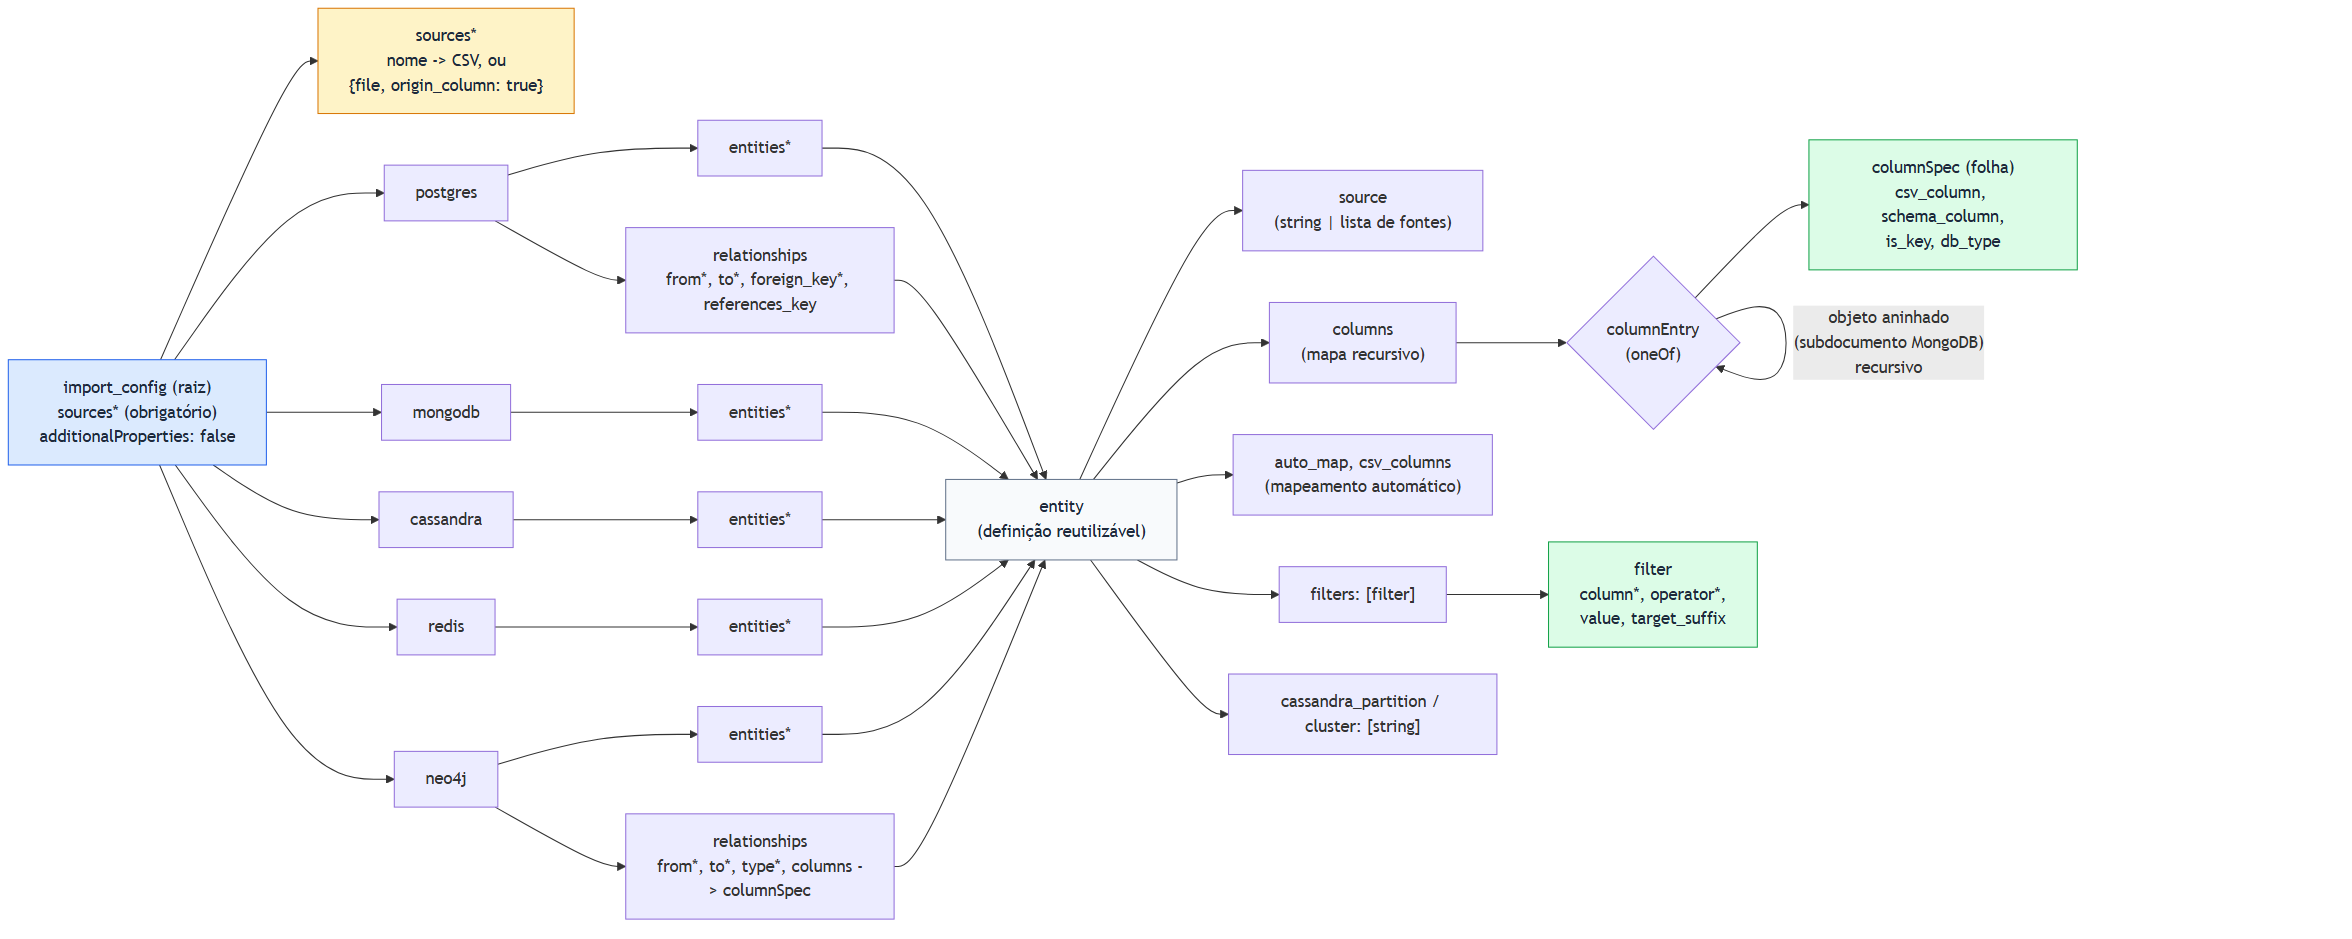
\includegraphics[width=\textwidth]{images/figure8-import-schema}
  \caption{Estrutura do JSON Schema de importação (\texttt{import\_config}).}
  \label{fig:import-schema}
  \par\vspace{4pt}
  {\footnotesize Fonte: Elaborado pelo autor (2026).}
\end{figure}

\begin{figure}[H]
  \centering
  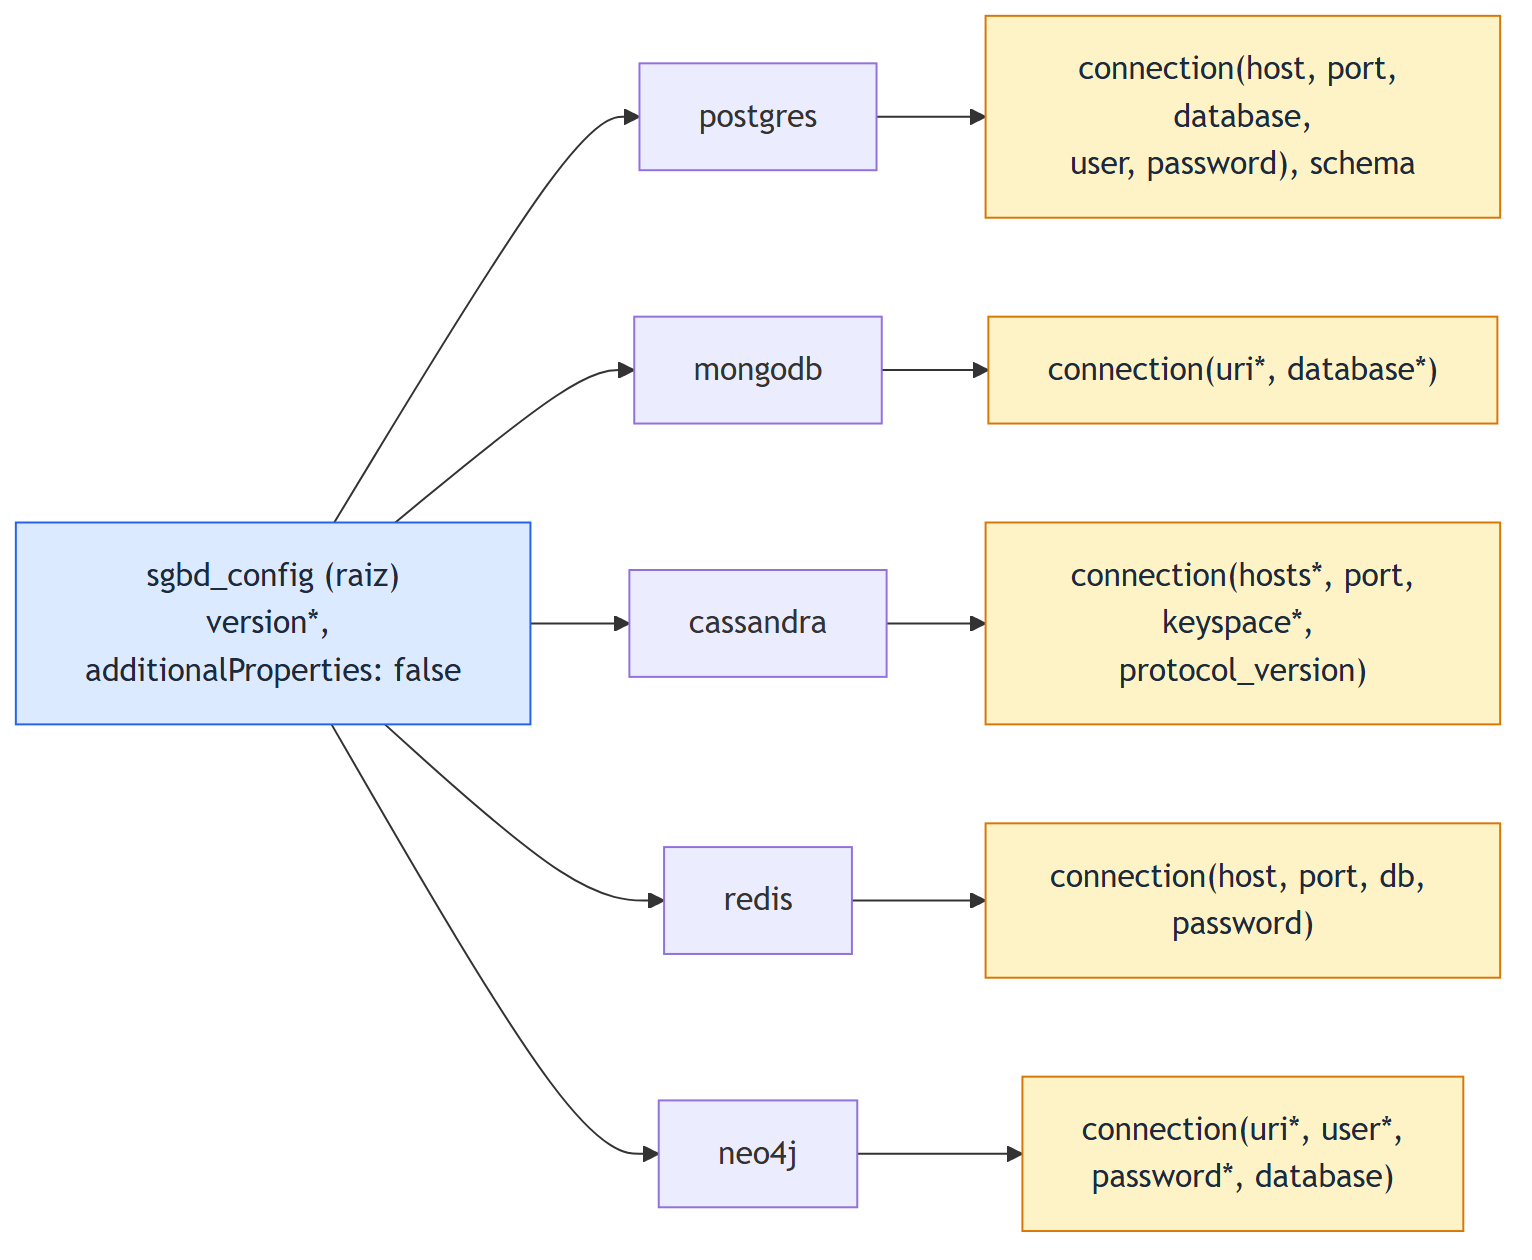
\includegraphics[width=0.85\textwidth]{images/figure9-sgbd-schema}
  \caption{Estrutura do JSON Schema de conexão (\texttt{sgbd\_config}).}
  \label{fig:sgbd-schema}
  \par\vspace{4pt}
  {\footnotesize Fonte: Elaborado pelo autor (2026).}
\end{figure}

\textbf{Raízes por SGBD.} Ambos os schemas partilham a mesma organização: um bloco
opcional por SGBD (\texttt{postgres}, \texttt{mongodb}, \texttt{cassandra},
\texttt{redis}, \texttt{neo4j}), com \texttt{additionalProperties: false} rejeitando
chaves desconhecidas. A diferença está no conteúdo de cada bloco e na raiz: o arquivo de
importação exige o bloco \texttt{sources} (seção~\ref{sec:sources}) e descreve \textit{o
que} mapear; o de conexão exige um campo \texttt{version} e descreve \textit{onde}
gravar.

\textbf{O arquivo de importação e a definição reutilizável \texttt{entity}.}
Seguindo as setas a partir de \texttt{import\_config}, cada bloco de SGBD
expande-se em um mapa \texttt{entities} (e, para PostgreSQL e Neo4j, também em
\texttt{relationships}). O ponto central da Figura~\ref{fig:import-schema} --- e da economia de
vocabulário do schema --- é que \textbf{todas as entidades, de todos os
SGBDs, convergem para uma única definição reutilizável}, rotulada
\texttt{entity}. Em vez de cinco formatos distintos, há apenas um: toda entidade
possui um mapa \texttt{columns} (o mapeamento de colunas) e campos opcionais como
\texttt{source} (o vínculo com a fonte, seção~\ref{sec:sources}), \texttt{auto\_map} e
\texttt{csv\_columns} (mapeamento automático, seção~\ref{sec:raiz}), \texttt{filters}
(predicados sobre as linhas) e os campos específicos do Cassandra
(\texttt{cassandra\_partition} e \texttt{cassandra\_cluster}).

\textbf{O mapeamento recursivo de colunas.} À direita da Figura~\ref{fig:import-schema}, \texttt{columns}
remete a \texttt{columnEntry}, definido como uma escolha (\texttt{oneOf}) entre duas
formas: (i) uma \textbf{folha} --- o \texttt{columnSpec}, que liga uma coluna do CSV
a um atributo do destino por meio dos campos \texttt{csv\_column},
\texttt{schema\_column}, \texttt{is\_key} e \texttt{db\_type}; ou (ii) um
\textbf{objeto aninhado}, que contém novos \texttt{columnEntry}. Essa recursão é o
que permite, com um único mecanismo, tanto o mapeamento plano (PostgreSQL,
Cassandra, Redis) quanto os subdocumentos do MongoDB. As arestas tipadas do Neo4j
e as chaves estrangeiras do PostgreSQL aparecem em \texttt{relationships},
reutilizando o mesmo \texttt{columnSpec} para eventuais propriedades.

\textbf{O arquivo de conexão.} Na Figura~\ref{fig:sgbd-schema}, cada bloco de
SGBD de \texttt{sgbd\_config} carrega apenas um descritor
\texttt{connection} com os parâmetros de acesso pertinentes àquela tecnologia (por
exemplo, \texttt{uri} para MongoDB e Neo4j; \texttt{hosts} e \texttt{keyspace} para
Cassandra). É uma estrutura deliberadamente rasa: indica \textit{onde} alcançar cada
SGBD, sem nenhuma informação de mapeamento.

As subseções seguintes percorrem essa estrutura na ordem em que as duas figuras são
lidas: primeiro a raiz e os elementos comuns a todos os SGBDs
(\texttt{columnSpec}, \texttt{entity}, mapeamento automático e filtros) e, em seguida, as
particularidades de cada SGBD, ilustradas com fragmentos concretos de configuração.

\subsection{Raiz e Elementos Comuns}
\label{sec:raiz}

Como antecipado na visão geral, ambos os arquivos organizam-se em um bloco opcional por
SGBD. A cláusula \texttt{additionalProperties: false} \textbf{rejeita} qualquer
propriedade não prevista, impedindo que erros de digitação como \texttt{postgress}
passem despercebidos.

\textbf{columnSpec.} Cada \textbf{folha} do mapa \texttt{columns} descreve como um valor
do CSV alimenta um atributo no destino. Quatro campos opcionais compõem esse mapeamento,
conforme a Tabela~\ref{tab:columnspec}.

\begin{table}[H]
  \caption{Campos de mapeamento de coluna (\texttt{columnSpec}).}
  \label{tab:columnspec}
  \centering
  \begin{tabular}{>{\ttfamily}l l l >{\raggedright\arraybackslash}p{5cm}}
    \toprule
    \normalfont\textbf{Campo} & \textbf{Tipo} & \textbf{Obrigatório} & \textbf{Descrição} \\
    \midrule
    csv\_column    & \textit{string} ou inteiro ($\geq 1$) & não & Cabeçalho CSV ou índice da coluna de dados (base 1). Padrão: chave JSON. \\
    schema\_column & \textit{string} & não & Nome do atributo no SGBD destino. Padrão: chave JSON. \\
    is\_key        & booleano & não & Chave primária, chave de \texttt{MERGE} (Neo4j) ou chave Redis. \\
    db\_type       & \textit{string} & não & Tipo SQL/CQL para geração de DDL. \\
    \bottomrule
  \end{tabular}
  \par\vspace{4pt}
  {\footnotesize Fonte: Elaborado pelo autor (2026).}
\end{table}

A chave JSON de cada entrada em \texttt{columns} identifica o mapeamento e serve de
\textbf{padrão} tanto para a coluna de origem no CSV quanto para o atributo de destino
no SGBD; por isso a forma mínima (\texttt{"campo": \{\}}) basta quando os três nomes
coincidem. Quando divergem, \texttt{csv\_column} redefine a origem --- por nome de
cabeçalho ou por índice posicional de base 1, útil para CSVs sem cabeçalho --- e
\texttt{schema\_column} redefine o destino no SGBD. Por ser um identificador
independente da origem, a chave permite ainda que uma mesma coluna do CSV alimente
atributos distintos (entradas com \texttt{csv\_column} repetido), recurso pontual para
cenários de denormalização.

\textbf{Mapeamento automático (\texttt{auto\_map} e \texttt{csv\_columns}).} Nem sempre é
prático enumerar coluna a coluna. Quando o campo \texttt{columns} é omitido, ou quando
\texttt{auto\_map} é \texttt{true}, a entidade \textbf{mapeia automaticamente} todas as
colunas da sua fonte, atribuindo a cada uma o nome e um tipo de destino inferido do
próprio dado (adiante, em \textbf{Inferência de tipos}); entradas manuais em
\texttt{columns} sobrepõem-se às automáticas coluna a coluna, permitindo, por exemplo,
declarar apenas a chave e deixar o restante ser inferido. O campo \texttt{csv\_columns}
--- válido apenas com mapeamento automático --- \textbf{restringe} o conjunto
auto-mapeado a colunas específicas, indicadas por nome, por índice de base 1 ou por
intervalos como \texttt{"1-5"}.

\textbf{Inferência de tipos.} Todos os valores são lidos inicialmente como texto,
preservando o conteúdo original do arquivo. Em seguida, a ferramenta classifica cada
coluna segundo o tipo predominante entre os seus valores --- inteiro, real, data/hora,
booleano, texto ou vazia --- e converte os valores para o tipo nativo correspondente.
Essa classificação também define o tipo de destino (\texttt{db\_type}) usado na geração de
DDL quando a coluna é auto-mapeada, segundo a correspondência da
Tabela~\ref{tab:kinds}.

\begin{table}[H]
  \caption{Correspondência entre tipo inferido e tipo de destino na geração de DDL.}
  \label{tab:kinds}
  \centering
  \begin{tabular}{l l}
    \toprule
    \textbf{Tipo inferido} & \textbf{Tipo de destino (\texttt{db\_type})} \\
    \midrule
    inteiro (\textit{integer})   & \texttt{BIGINT} \\
    real (\textit{float})        & \texttt{NUMERIC} \\
    data/hora (\textit{datetime}) & \texttt{TIMESTAMPTZ} \\
    booleano (\textit{boolean})  & \texttt{BOOLEAN} \\
    texto (\textit{string}) ou vazia & \texttt{TEXT} \\
    \bottomrule
  \end{tabular}
  \par\vspace{4pt}
  {\footnotesize Fonte: Elaborado pelo autor (2026).}
\end{table}

\textbf{entity.} Uma entidade representa um alvo lógico: tabela (PostgreSQL/Cassandra),
coleção (MongoDB), rótulo de nó (Neo4j) ou entidade Redis. O único campo estritamente
necessário é o vínculo com a fonte (explícito em \texttt{source} ou implícito pelo nome);
\texttt{columns} pode ser omitido em favor do mapeamento automático. São opcionais
\texttt{auto\_map} e \texttt{csv\_columns} (mapeamento automático), \texttt{filters}
(predicados sobre as linhas), e \texttt{cassandra\_partition} e
\texttt{cassandra\_cluster} (apenas Cassandra).

\textbf{Filtros.} Além do vínculo com a fonte, uma entidade pode declarar
\texttt{filters}: predicados opcionais que \textbf{restringem} as linhas participantes.
Cada item exige \texttt{column} e \texttt{operator} (\texttt{==}, \texttt{!=},
\texttt{>}, \texttt{<}, \texttt{>=}, \texttt{<=}, \texttt{in}, \texttt{not\_in},
\texttt{each}). O operador \texttt{each} particiona a entidade por valores distintos da
coluna, gerando múltiplos alvos com sufixo opcional. Diferentemente da seleção da origem
--- feita pelo bloco \texttt{sources} e pelo campo \texttt{source} ---, os filtros são um
refinamento adicional; no cenário de e-commerce, em que cada assunto já vem de uma fonte
própria, eles não são necessários e não aparecem na configuração.

\subsection{PostgreSQL}

\textbf{Arquivo de importação.} O bloco \texttt{postgres} contém \texttt{entities}
(entidades planas --- aninhamento de \texttt{columns} é rejeitado) e, opcionalmente,
\texttt{relationships} para declarar chaves estrangeiras. O campo \texttt{db\_type} em
cada \texttt{columnSpec} alimenta a geração de DDL (\texttt{CREATE TABLE}) quando
\texttt{-{}-create-schema} está ativo. A Listagem~\ref{lst:pg-import} mostra um fragmento
da importação no domínio de e-commerce.

\begin{lstlisting}[style=jsonstyle,caption={Fragmento de importação PostgreSQL (e-commerce).},label={lst:pg-import}]
"postgres": {
  "entities": {
    "inventory": {
      "source": "stock",
      "columns": {
        "product_id":         { "is_key": true, "db_type": "BIGINT" },
        "quantity_available": { "db_type": "BIGINT" },
        "last_restock_date":  { "db_type": "TIMESTAMPTZ" },
        "price":              { "db_type": "NUMERIC(14,2)" }
      }
    },
    ...
  },
  "relationships": {
    "product_category": {
      "from": "products",
      "to":   "categories",
      "foreign_key":    "category_id",
      "references_key": "category_id"
    },
    ...
  }
}
\end{lstlisting}

As reticências indicam que o arquivo real declara outras três entidades
(\texttt{categories}, \texttt{products} e \texttt{orders}) e uma segunda chave
estrangeira (\texttt{order\_product}), omitidas aqui por brevidade; o arquivo
completo é reproduzido no Apêndice~\ref{ap:config}. O campo \texttt{source} liga a
entidade \texttt{inventory} à fonte \texttt{stock} (as linhas de reposição de estoque),
das quais projeta quatro colunas, com \texttt{product\_id} como chave.

\textbf{Arquivo de conexão.} O bloco \texttt{postgres} contém \texttt{connection}
(host, port, database, user, password) e o campo \texttt{schema} (padrão
\texttt{public}), que define o schema PostgreSQL de destino das tabelas. A
Listagem~\ref{lst:pg-conn} mostra um exemplo de configuração de conexão.

\begin{lstlisting}[style=jsonstyle,caption={Fragmento de conexão PostgreSQL.},label={lst:pg-conn}]
"postgres": {
  "connection": {
    "host": "127.0.0.1", "port": 5432,
    "database": "ecommerce",
    "user": "postgres", "password": "postgres"
  },
  "schema": "public"
}
\end{lstlisting}

\subsection{MongoDB}

\textbf{Arquivo de importação.} O bloco \texttt{mongodb} contém apenas
\texttt{entities}. O diferencial do MongoDB é o suporte a
\textbf{aninhamento de \texttt{columns}}: chaves JSON aninhadas produzem subdocumentos
BSON, sem necessidade de nenhum campo adicional --- o próprio mapa recursivo expressa a
hierarquia. A Listagem~\ref{lst:mongo-import} exemplifica esse aninhamento: as chaves
\texttt{category} e \texttt{stock} não são colunas do CSV, e sim objetos que agrupam
outras colunas, produzindo dois subdocumentos dentro de cada documento
\texttt{product\_catalog}, também alimentado pela fonte \texttt{stock}.

\begin{lstlisting}[style=jsonstyle,caption={Fragmento de importação MongoDB com subdocumentos.},label={lst:mongo-import}]
"mongodb": {
  "entities": {
    "product_catalog": {
      "source": "stock",
      "columns": {
        "product_id":   {},
        "product_name": {},
        ...
        "category": {
          "category_id": {},
          "category_name": {}
        },
        "stock": {
          "quantity_available": {},
          "last_restock_date": {}
        }
      }
    }
  }
}
\end{lstlisting}

As reticências omitem as demais colunas cadastrais do produto (variante, marca,
descrição, imagem e preço), mapeadas de forma direta como \texttt{product\_id} e
\texttt{product\_name}; o bloco completo encontra-se no Apêndice~\ref{ap:config}.

\textbf{Arquivo de conexão.} O bloco \texttt{mongodb} contém \texttt{connection}
com \texttt{uri} (string de conexão MongoDB, incluindo usuário e senha quando
necessário) e \texttt{database} (nome do banco de destino), como na
Listagem~\ref{lst:mongo-conn}.

\begin{lstlisting}[style=jsonstyle,caption={Fragmento de conexão MongoDB.},label={lst:mongo-conn}]
"mongodb": {
  "connection": {
    "uri": "mongodb://127.0.0.1:27017",
    "database": "ecommerce"
  }
}
\end{lstlisting}

\subsection{Apache Cassandra}

\textbf{Arquivo de importação.} O bloco \texttt{cassandra} contém \texttt{entities}
planas. Dois campos específicos controlam a chave primária composta do Cassandra:
\texttt{cassandra\_\allowbreak partition} (lista de colunas que formam a chave de partição)
e \texttt{cassandra\_\allowbreak cluster} (colunas de agrupamento). O campo
\texttt{cassandra\_\allowbreak partition} é obrigatório para gerar o schema Cassandra:
sua ausência só é detectada quando \texttt{-{}-create-schema} está ativo, pois o CQL
exige ao menos uma coluna de partição na cláusula \texttt{PRIMARY KEY}; esse campo é
independente de \texttt{is\_key}, que no Cassandra não tem papel na definição da chave
primária. A Listagem~\ref{lst:cassandra-import} ilustra uma entidade que \textbf{une}
todas as fontes e usa uma chave composta.

\begin{lstlisting}[style=jsonstyle,caption={Fragmento de importação Cassandra com união de fontes e chave composta.},label={lst:cassandra-import}]
"cassandra": {
  "entities": {
    "user_activity_log": {
      "source": ["stock", "purchase", "select_product", "add_to_cart"],
      "columns": {
        "user_id":             {},
        "timestamp":           { "schema_column": "event_time" },
        "_source":             { "schema_column": "event_type" },
        "product_id":          {},
        "order_number":        {},
        "selected_product_id": {},
        "shopping_cart_id":    {}
      },
      "cassandra_partition": ["user_id"],
      "cassandra_cluster":   ["timestamp"]
    }
  }
}
\end{lstlisting}

A entidade \texttt{user\_activity\_log} declara \texttt{source} como a \textbf{lista} das
quatro fontes: as suas linhas são unidas em uma única tabela de eventos. A pseudo-coluna
\texttt{\_source} --- que registra a origem de cada linha --- é mapeada para a coluna
\texttt{event\_type}, distinguindo os tipos de evento na tabela CQL; de modo análogo,
\texttt{schema\_column} renomeia \texttt{timestamp} para \texttt{event\_time}. É um exemplo
concreto de como \texttt{csv\_column}/\texttt{\_source} e \texttt{schema\_column} atuam
independentemente.

\textbf{Arquivo de conexão.} O bloco \texttt{cassandra} contém \texttt{connection}
com \texttt{hosts} (lista de endereços de nós), \texttt{port} (padrão 9042),
\texttt{keyspace} e \texttt{protocol\_version} opcional, conforme a
Listagem~\ref{lst:cassandra-conn}.

\begin{lstlisting}[style=jsonstyle,caption={Fragmento de conexão Cassandra.},label={lst:cassandra-conn}]
"cassandra": {
  "connection": {
    "hosts": ["127.0.0.1"],
    "port": 9042,
    "keyspace": "ecommerce"
  }
}
\end{lstlisting}

\subsection{Redis}

\textbf{Arquivo de importação.} O bloco \texttt{redis} contém \texttt{entities}.
A restrição fundamental é que \textbf{cada entidade deve ter exatamente uma coluna
marcada com \texttt{is\_key}}: esse valor se torna a chave Redis --- usada exatamente
como aparece no CSV --- e todos os demais campos mapeados compõem o valor JSON
armazenado. A Listagem~\ref{lst:redis-import} mostra as duas entidades do cenário
e-commerce e ilustra o mapeamento automático: \texttt{shopping\_cart} declara apenas a
chave e usa \texttt{auto\_map} para mapear todas as demais colunas da fonte
\texttt{add\_to\_cart}.

\begin{lstlisting}[style=jsonstyle,caption={Fragmento de importação Redis (e-commerce), com mapeamento automático.},label={lst:redis-import}]
"redis": {
  "entities": {
    "shopping_cart": {
      "source": "add_to_cart",
      "auto_map": true,
      "columns": {
        "shopping_cart_id": { "is_key": true }
      }
    },
    "user_session": {
      "source": "select_product",
      "columns": {
        "user_id":    { "is_key": true },
        "user_name":  {},
        "user_email": {},
        "timestamp":  { "schema_column": "last_seen" }
      }
    }
  }
}
\end{lstlisting}

A entidade \texttt{shopping\_cart} lê da fonte \texttt{add\_to\_cart} e usa como chave o
identificador do carrinho (\texttt{shopping\_cart\_id}); com \texttt{auto\_map}, o valor
armazenado reúne automaticamente as demais colunas da fonte. A entidade
\texttt{user\_session} lê da fonte \texttt{select\_product}, usa como chave o
identificador do usuário e renomeia \texttt{timestamp} para \texttt{last\_seen},
registrando a última atividade de navegação de cada usuário.

\textbf{Arquivo de conexão.} O bloco \texttt{redis} contém \texttt{connection}
com \texttt{host}, \texttt{port} (padrão 6379), \texttt{db} (índice do banco,
padrão 0) e \texttt{password} opcional, como na Listagem~\ref{lst:redis-conn}.

\begin{lstlisting}[style=jsonstyle,caption={Fragmento de conexão Redis.},label={lst:redis-conn}]
"redis": {
  "connection": {
    "host": "127.0.0.1",
    "port": 6379,
    "db": 0
  }
}
\end{lstlisting}

\subsection{Neo4j}

\textbf{Arquivo de importação.} O bloco \texttt{neo4j} contém \texttt{entities}
(nós) e \texttt{relationships} (arestas tipadas). Cada entidade declara um rótulo
(\textit{label}) de nó e deve ter exatamente uma coluna \texttt{is\_key}, usada como
predicado de identificação no \texttt{MERGE} Cypher. As arestas em
\texttt{relationships} declaram \texttt{from} (rótulo de origem), \texttt{to}
(rótulo de destino), \texttt{type} (tipo da aresta em maiúsculas) e um mapa
\texttt{columns} opcional com propriedades da aresta. A Listagem~\ref{lst:neo4j-import}
mostra um nó de cada rótulo, ligados por uma aresta.

\begin{lstlisting}[style=jsonstyle,caption={Fragmento de importação Neo4j (nós e aresta).},label={lst:neo4j-import}]
"neo4j": {
  "entities": {
    "User": {
      "source": "purchase",
      "columns": {
        "user_id":    { "is_key": true },
        "user_name":  {},
        "user_email": {}
      }
    },
    "Product": {
      "source": "stock",
      "columns": {
        "product_id":    { "is_key": true },
        "product_name":  {},
        "product_brand": {}
      }
    }
  },
  "relationships": {
    "PURCHASED": {
      "from": "User",
      "to":   "Product",
      "type": "PURCHASED",
      "columns": {
        "order_number": { "is_key": true },
        "quantity":     {},
        "price":        {},
        "rating":       {}
      }
    }
  }
}
\end{lstlisting}

O nó \texttt{User} lê da fonte \texttt{purchase} (os compradores) e o nó \texttt{Product},
da fonte \texttt{stock} (os produtos repostos); a aresta \texttt{PURCHASED} liga um ao
outro pela fonte de origem (\texttt{purchase}), decorada com quantidade, preço e nota da
avaliação.

\textbf{Arquivo de conexão.} O bloco \texttt{neo4j} contém \texttt{connection}
com \texttt{uri} (bolt://\ldots), \texttt{user}, \texttt{password} e
\texttt{database} opcional (padrão \texttt{neo4j}), conforme a
Listagem~\ref{lst:neo4j-conn}.

\begin{lstlisting}[style=jsonstyle,caption={Fragmento de conexão Neo4j.},label={lst:neo4j-conn}]
"neo4j": {
  "connection": {
    "uri":      "bolt://127.0.0.1:7687",
    "user":     "neo4j",
    "password": "password",
    "database": "neo4j"
  }
}
\end{lstlisting}

\subsection{Validação, Consistência entre Arquivos e Fluxo de Carregamento}
\label{sec:validacao}

A validação ocorre em \textbf{três camadas} antes de qualquer conexão com os SGBDs. A
primeira é a validação por \textbf{JSON Schema}: cada arquivo é validado contra o seu
schema (sintaxe, tipos e propriedades permitidas) --- \texttt{import\_config.schema.json}
para o arquivo de importação e \texttt{sgbd\_config.schema.json} para o arquivo de
conexão. A segunda é a \textbf{consistência entre arquivos}
(\texttt{config\_parser.merge\_configs}): todo SGBD referenciado no arquivo
de importação deve estar declarado no arquivo de conexão. A terceira é a
\textbf{validação cruzada com os dados}: ao carregar as fontes
(\texttt{sources.load\_sources}) e vincular cada entidade à sua fonte
(\texttt{mapping\_resolver}), confere-se se as colunas referenciadas existem, se os SGBDs
de modelo plano não usam \texttt{columns} aninhados, se as colunas de partição e
agrupamento do Cassandra existem, se os filtros são coerentes e se as chaves estrangeiras
do PostgreSQL e as arestas do Neo4j referenciam entidades válidas
(\texttt{validation.validate\_backend\_entities}).

Cada camada levanta uma exceção específica da hierarquia \texttt{BusinessException}, o que
torna o diagnóstico preciso: \texttt{ConfigError} para erros de schema ou de consistência
entre os arquivos; \texttt{SourceError} para problemas com os arquivos de fonte (por
exemplo, um CSV inexistente ou uma coluna de origem vazia no modo combinado);
\texttt{MappingError} para incoerências entre o mapeamento e os dados; e
\texttt{ImportExecutionError} para falhas na conexão ou na gravação em um SGBD. Qualquer
falha nas três primeiras camadas \textbf{impede} o início da importação. A
Figura~\ref{fig:config-pipeline} apresenta o fluxo completo de carregamento, com os
pontos de falha de cada camada e a convergência dos dois arquivos em uma configuração
única, à qual os dados das fontes se juntam apenas na validação cruzada (camada 3). O
diagrama evidencia por que a separação em dois arquivos isola falhas: um
\texttt{sgbd\_config.json} inválido é detectado independentemente do
\texttt{import\_config.json}, sem necessidade de ler os CSVs.

\begin{figure}[H]
  \centering
  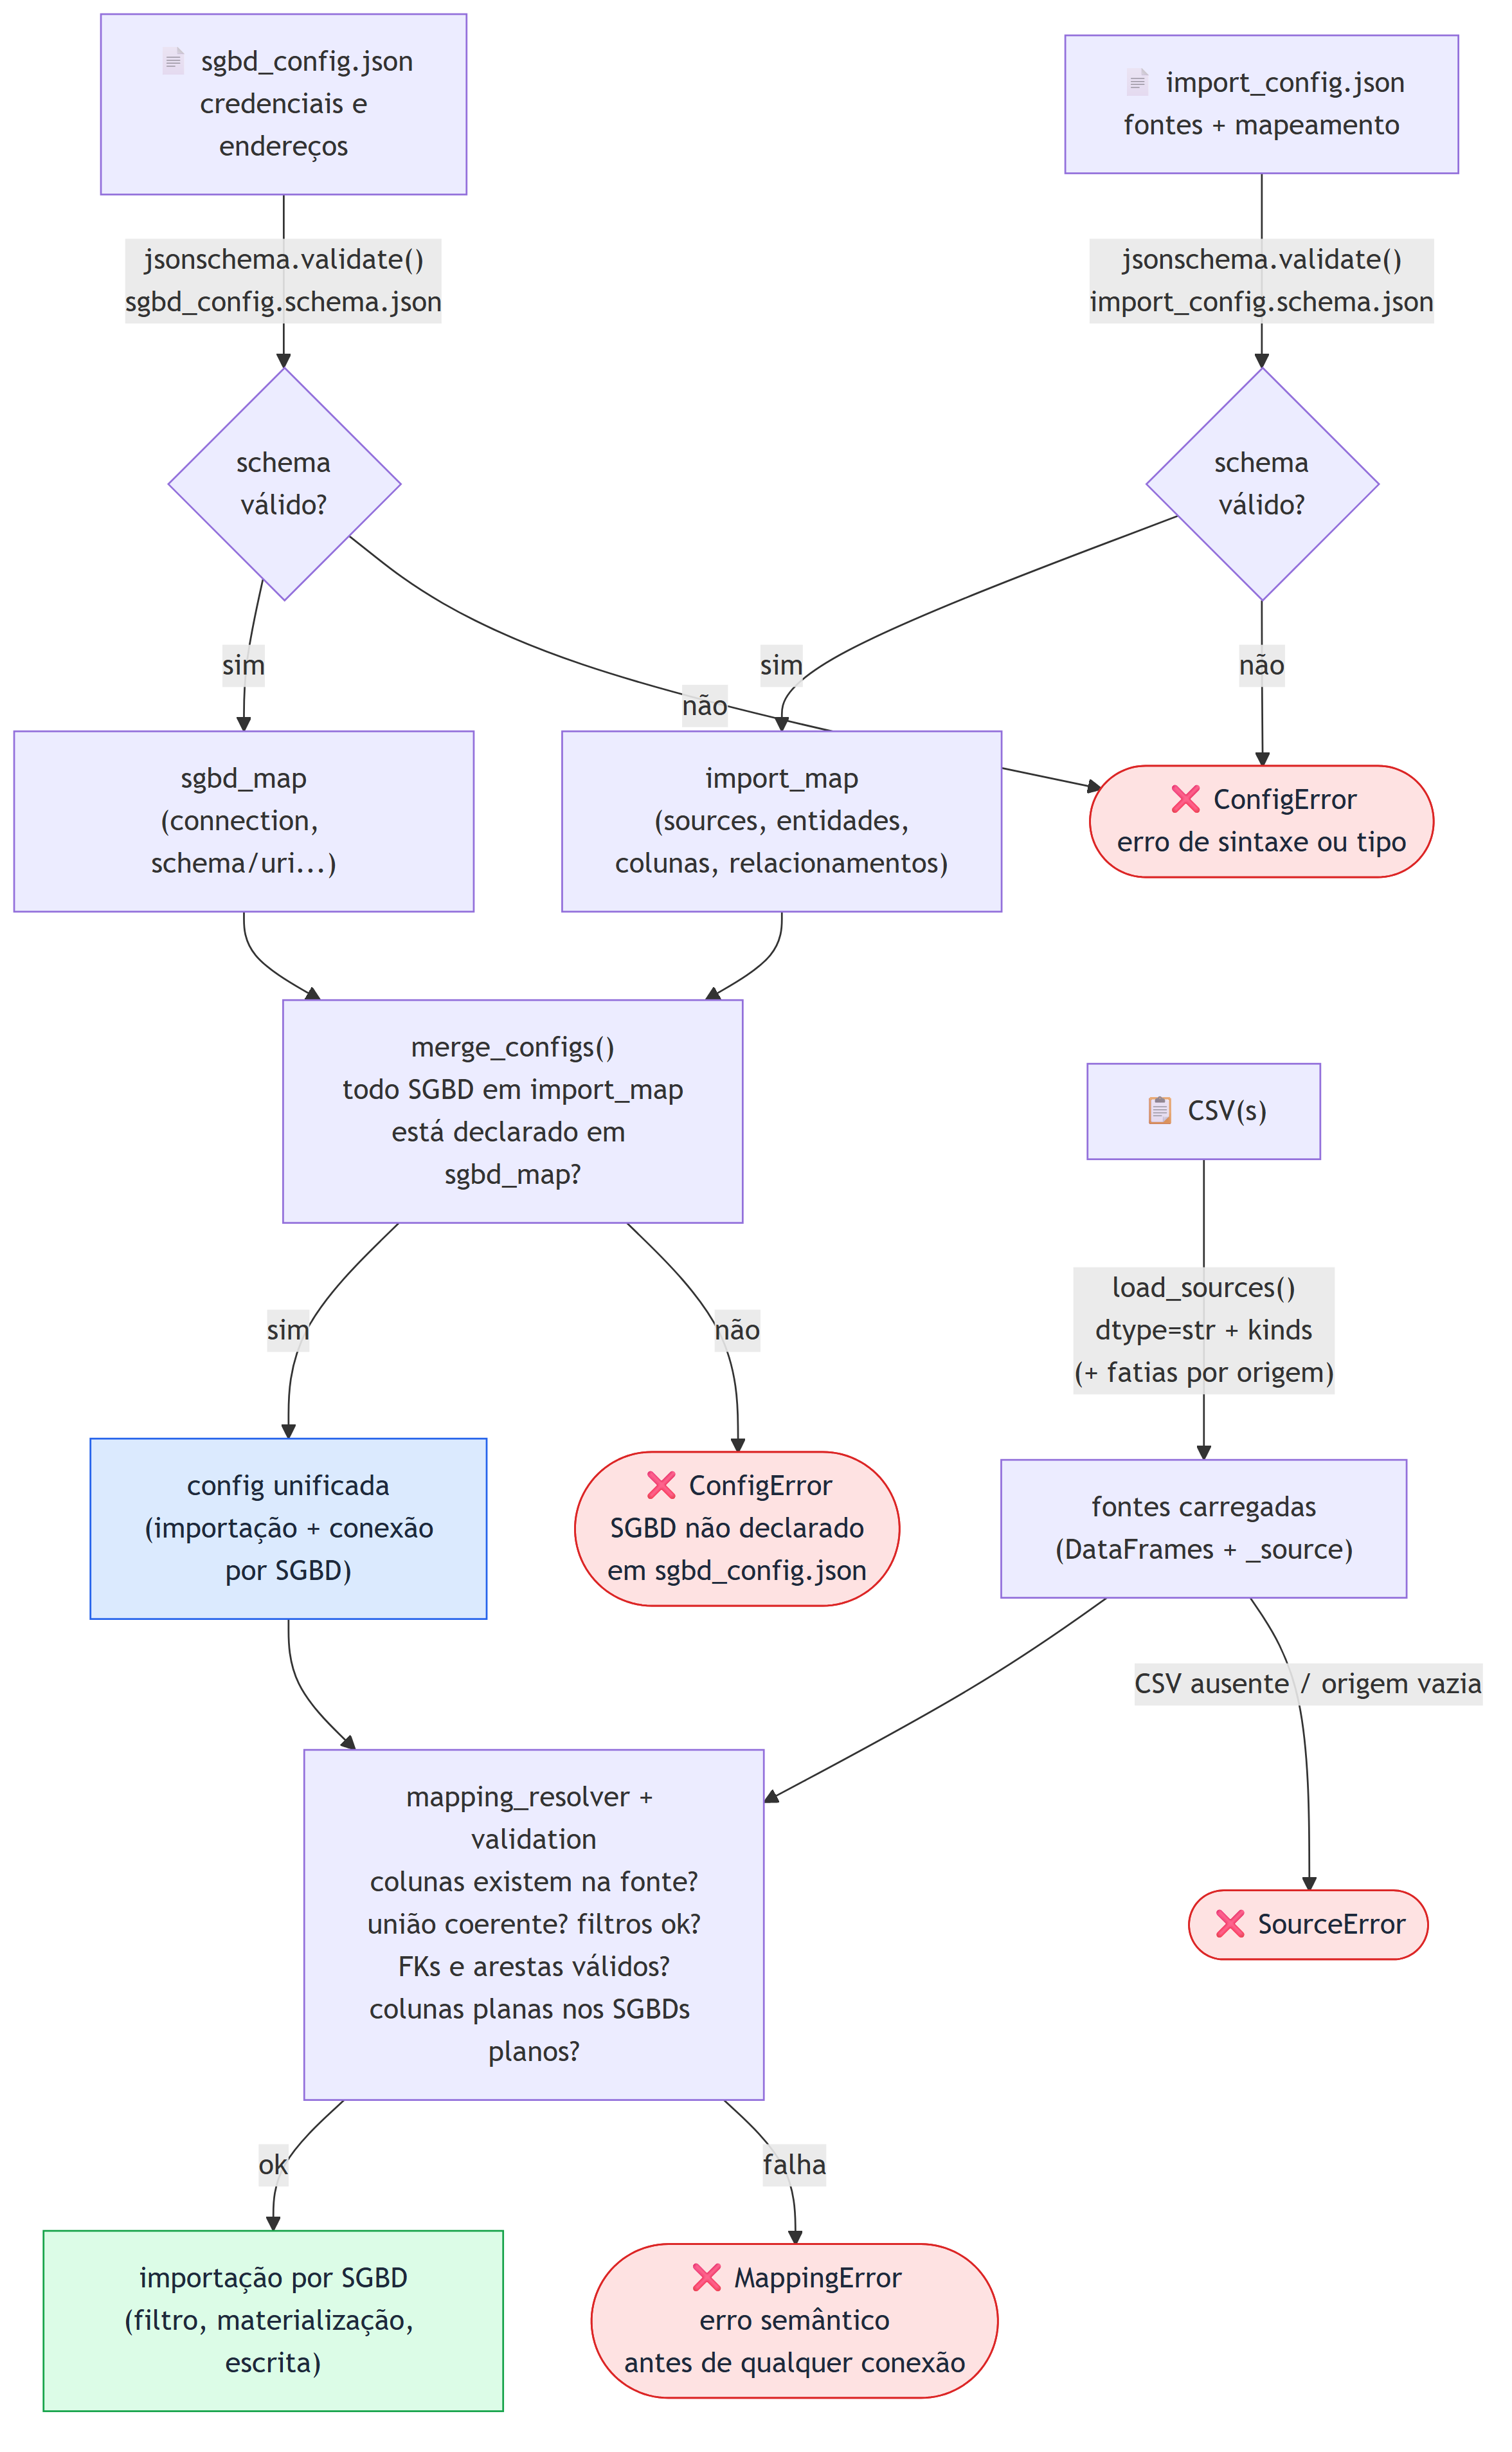
\includegraphics[width=14cm]{images/figure10-config-pipeline}
  \caption{Fluxo de carregamento e validação das entradas da ferramenta.}
  \label{fig:config-pipeline}
  \par\vspace{4pt}
  {\footnotesize Fonte: Elaborado pelo autor (2026).}
\end{figure}

\section{Algoritmo de Execução da Importação}
\label{sec:algoritmo}

Definidos o formato de configuração e as validações, esta seção descreve como a
ferramenta executa a importação propriamente dita, desde o comando de linha de comando
apresentado na seção~\ref{sec:visao-geral} até a persistência em cada SGBD. A
Figura~\ref{fig:import-algorithm} apresenta o fluxo completo de execução; cada etapa do
diagrama é explicada textualmente na sequência.

\begin{figure}[H]
  \centering
  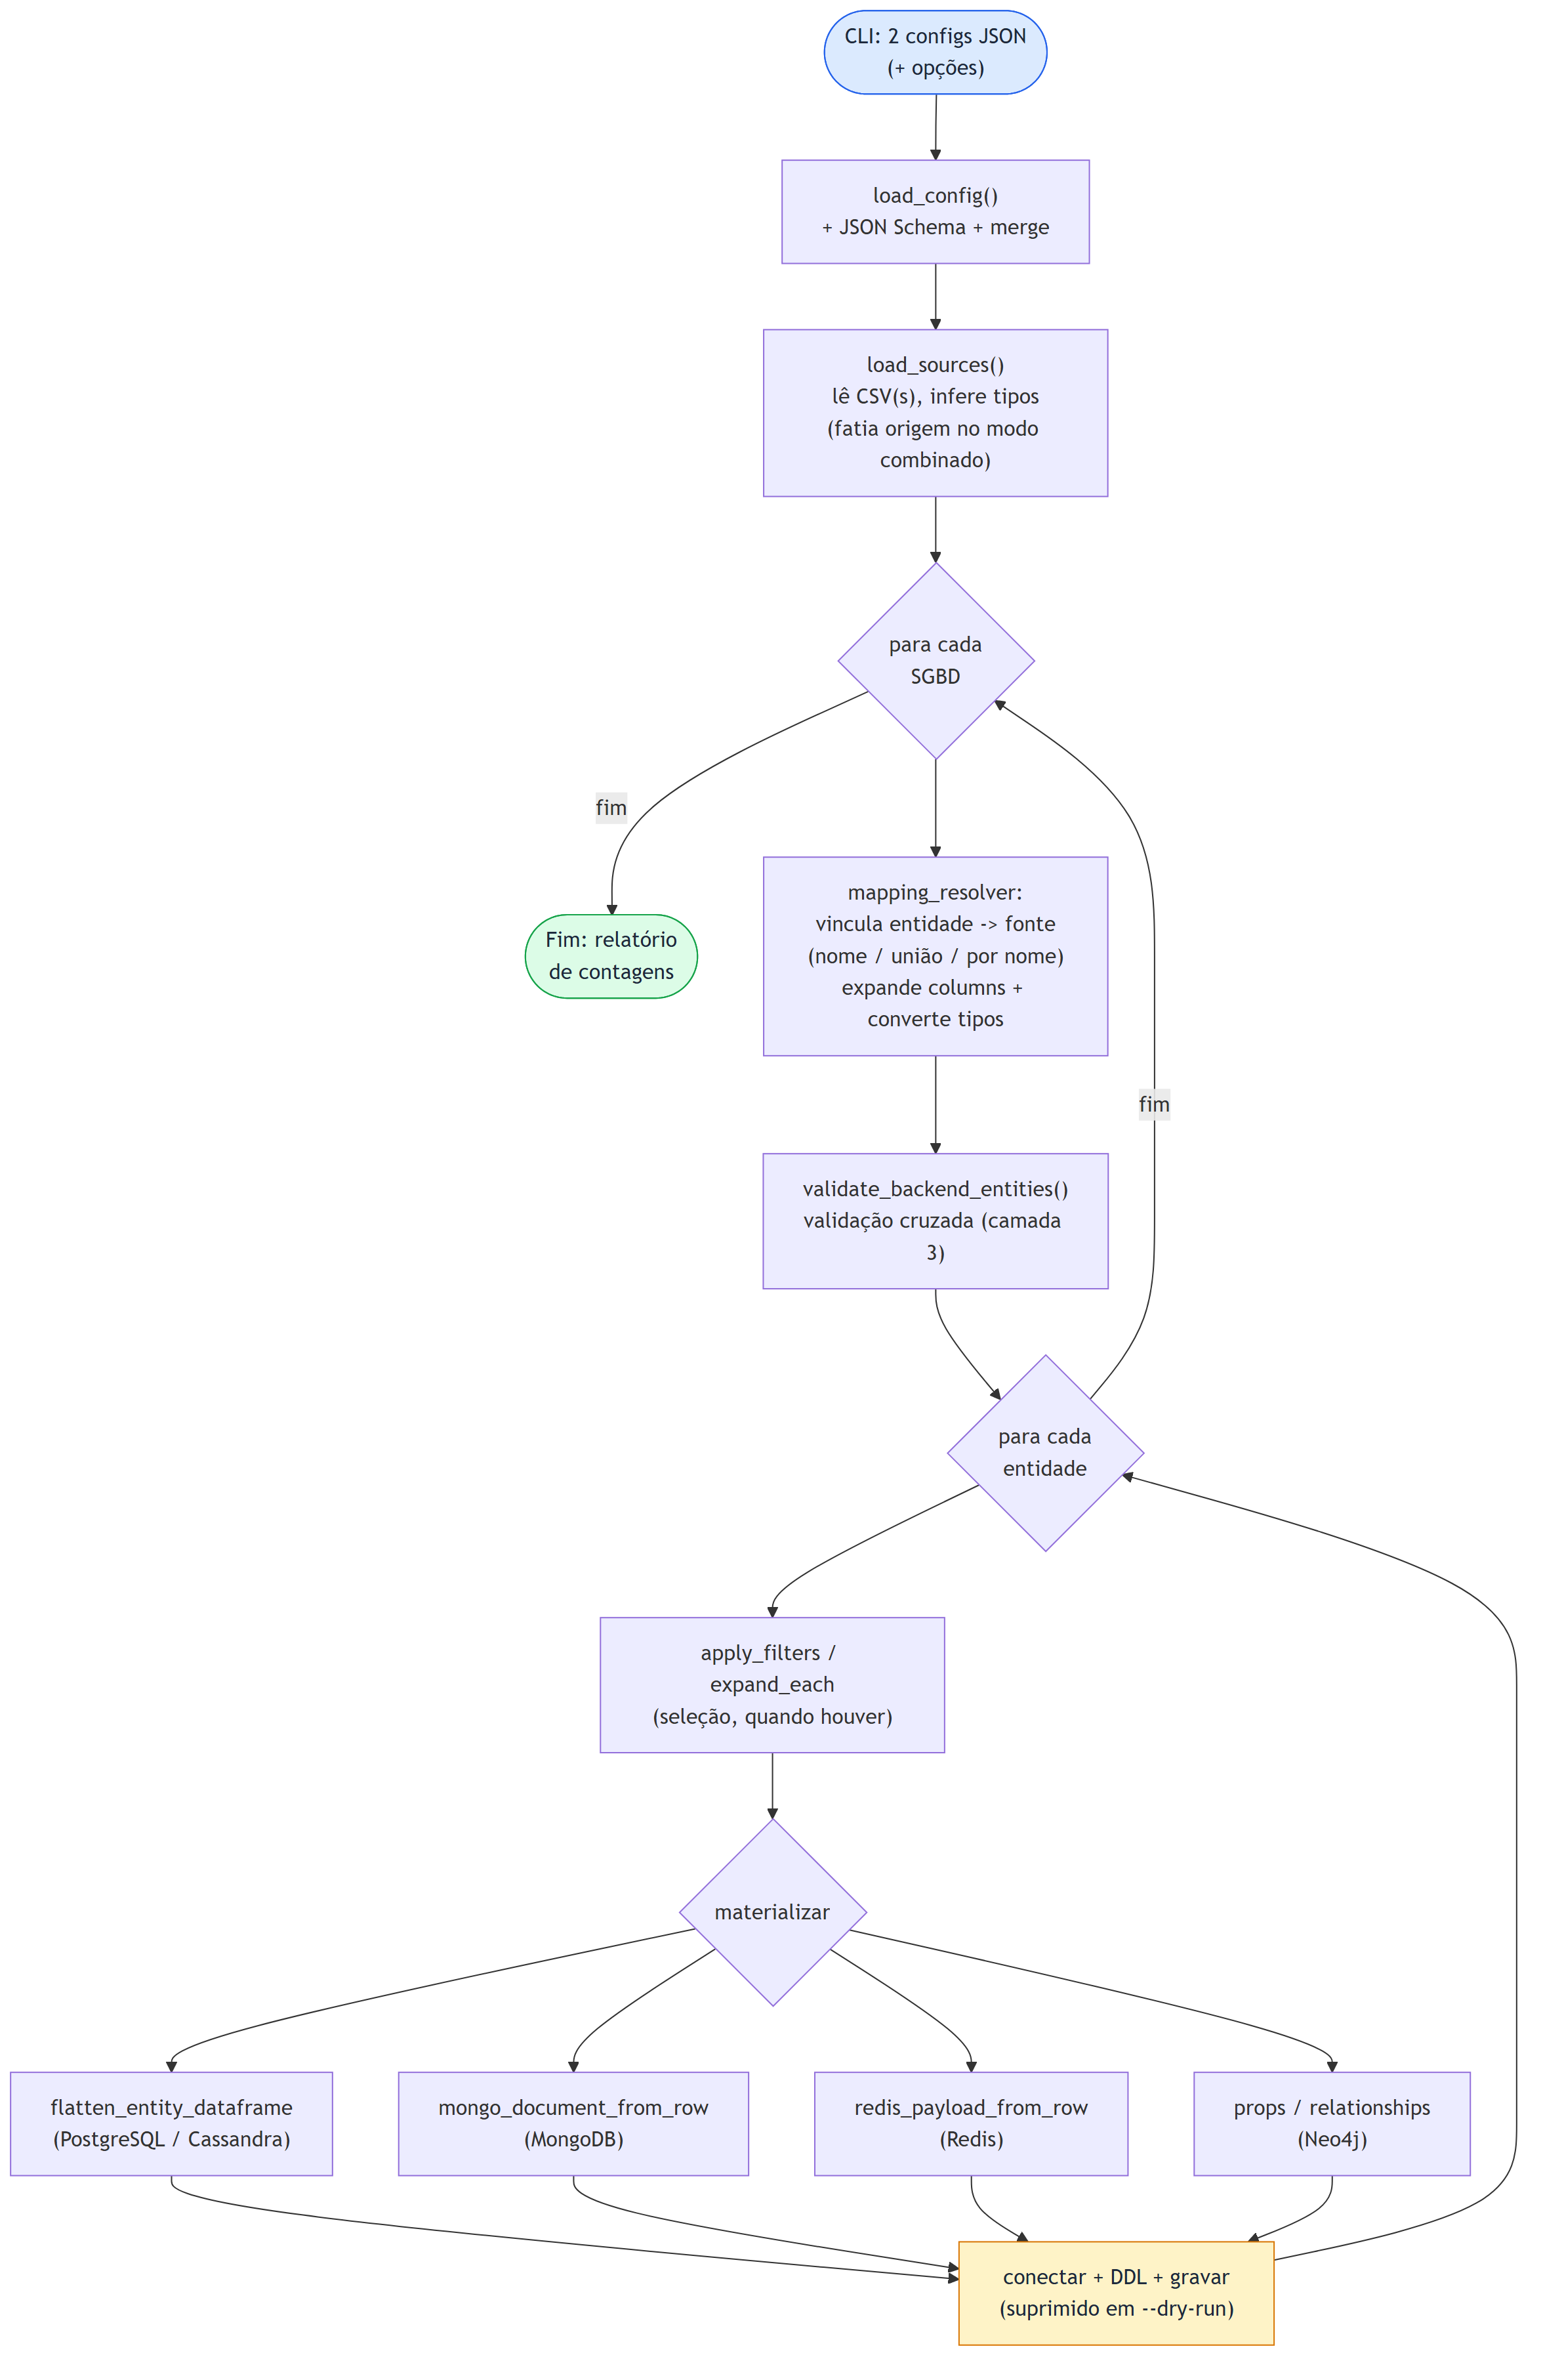
\includegraphics[width=12cm]{images/figure11-import-algorithm}
  \caption{Algoritmo de execução da importação PolyglotImportCSV.}
  \label{fig:import-algorithm}
  \par\vspace{4pt}
  {\footnotesize Fonte: Elaborado pelo autor (2026).}
\end{figure}

A execução parte da \textbf{entrada} fornecida pelo usuário na linha de comando: os
caminhos dos dois arquivos JSON de configuração (importação e conexão), eventuais
sobrescritas de fonte (\texttt{-{}-source}) e as opções de execução
\texttt{-{}-dry-run}, \texttt{-{}-create-schema}/\texttt{-{}-no-create-schema} e
\texttt{-{}-only}, descritas na seção~\ref{sec:visao-geral}.

Na etapa de \textbf{carregamento da configuração}, os dois arquivos JSON são lidos e
validados contra os seus respectivos JSON Schemas (camada 1 da
seção~\ref{sec:validacao}); em seguida, verifica-se a consistência entre os arquivos ---
todo SGBD referenciado no arquivo de importação deve estar declarado no
arquivo de conexão (camada 2) --- e as configurações são mescladas em uma estrutura única
de execução.

Na etapa de \textbf{carregamento das fontes}, cada CSV declarado no bloco
\texttt{sources} é lido uma única vez. Todos os valores são lidos inicialmente como
texto, preservando o conteúdo original do arquivo e evitando conversões prematuras de
tipo (por exemplo, em datas com fuso horário). Quando a fonte é combinada, a sua primeira
coluna é interpretada como a origem e cada valor distinto dá origem a uma fonte derivada;
a pseudo-coluna \texttt{\_source} é preenchida em ambos os modos. Em seguida, a ferramenta
infere o tipo de cada coluna de cada fonte, informação que alimenta tanto a conversão dos
valores para tipos nativos quanto a geração de DDL para colunas auto-mapeadas.

Validadas as entradas, inicia-se o núcleo do algoritmo, que percorre os SGBDs presentes
na configuração (excluídos os não selecionados por \texttt{-{}-only}) e, para cada um,
\textbf{vincula} as suas entidades às respectivas fontes (\texttt{mapping\_resolver}):
resolve o \texttt{source} de cada entidade --- nome único, união de fontes ou vínculo pelo
nome ---, expande o mapeamento de colunas (manual, automático ou híbrido) e converte os
valores da fonte para tipos nativos. Realiza-se então a validação cruzada da camada 3
(seção~\ref{sec:validacao}). Qualquer falha, em qualquer camada, encerra a execução com
uma mensagem de erro antes que qualquer conexão com os SGBDs seja aberta.

Para cada entidade vinculada, a ferramenta \textbf{aplica os filtros} declarados na
configuração, quando houver --- operação que corresponde à \textit{seleção} da álgebra
relacional: apenas as linhas que satisfazem os predicados participam da entidade. Havendo
filtro com o operador \texttt{each}, a entidade é adicionalmente \textbf{particionada}
pelos valores distintos da coluna indicada --- um particionamento horizontal em que cada
valor dá origem a um destino próprio, identificado por sufixo.

Em seguida, na \textbf{materialização}, cada linha selecionada é convertida na estrutura
do modelo de dados de destino, segundo os conceitos revisados no capítulo~2. Para os
SGBDs de organização tabular (o relacional PostgreSQL e o colunar Cassandra), a conversão
combina três operações também descritas pela álgebra relacional: \textit{projeção}
(somente as colunas mapeadas em \texttt{columns} são mantidas), \textit{renomeação}
(aplicação de \texttt{schema\_column}) e \textit{eliminação de duplicatas} com base nas
colunas de chave (\texttt{is\_key}), de modo que cada tabela receba apenas tuplas únicas.
Para o modelo de documentos (MongoDB), os valores da linha são agregados em um documento
cuja hierarquia reproduz o aninhamento declarado em \texttt{columns}, materializando a
representação desnormalizada característica desse modelo. Para o modelo chave-valor
(Redis), cada linha dá origem a um par em que a chave é o valor da coluna marcada com
\texttt{is\_key} e o valor é a representação textual (JSON) dos demais campos mapeados.
Para o modelo de grafo (Neo4j), cada linha dá origem a um nó com as propriedades mapeadas;
na sequência, as arestas declaradas em \texttt{relationships} conectam os nós criados, com
semântica de mesclagem --- a aresta só é criada se ainda não existir, evitando duplicação
quando a mesma relação aparece em várias linhas.

Por fim, para cada entidade materializada, a ferramenta \textbf{conecta-se} ao SGBD
(etapa suprimida quando \texttt{-{}-dry-run} está ativo), \textbf{cria as estruturas de
armazenamento} quando \texttt{-{}-create-schema} está ativo (tabelas no PostgreSQL;
\textit{keyspace} e tabelas no Cassandra) e \textbf{grava} os registros por meio da
operação de escrita própria de cada tecnologia. A \textbf{saída} da execução é um
relatório com as contagens de registros gravados por entidade e por SGBD, que permite
conferir o resultado da carga.

\subsection{O Cenário de Exemplo e os Arquivos de Dados}
\label{sec:exemplo-linha}

Para concretizar o algoritmo, esta subseção e a seguinte percorrem o cenário de
e-commerce que acompanha o repositório da ferramenta --- o mesmo cenário cujos
fragmentos de configuração ilustraram a seção~\ref{sec:config-format} e cuja execução
completa é demonstrada na seção~\ref{sec:exemplo-uso}.

Os dados do cenário registram os eventos de uma loja virtual, agrupados por tipo:
\textbf{reposição de estoque} (\texttt{stock}), \textbf{compra} (\texttt{purchase}),
\textbf{seleção de produto} (\texttt{select\_product}) e \textbf{adição ao carrinho}
(\texttt{add\_to\_cart}). No modo multifonte --- adotado como referência neste exemplo ---
cada tipo tem o seu próprio CSV (\texttt{ecommerce\_stock.csv},
\texttt{ecommerce\_purchase.csv}, \texttt{ecommerce\_select\_product.csv} e
\texttt{ecommerce\_add\_to\_cart.csv}), cada um com oito linhas e as colunas pertinentes
ao seu assunto. Como alternativa equivalente, o modo combinado reúne os mesmos eventos em
um único arquivo largo, \texttt{ecommerce\_join.csv}, cuja primeira coluna
(\texttt{action}) rotula a origem de cada linha; o Apêndice~\ref{ap:csv} reproduz esse
arquivo em forma tabular, organizado por ação.

A Tabela~\ref{tab:csv-stock} apresenta as oito linhas da fonte \texttt{stock}
(\texttt{ecommerce\_stock.csv}), que servem de fio condutor do exemplo. Para caber na
página, a tabela resume as colunas de identificação, cujos valores seguem padrões
regulares no arquivo: o produto \texttt{Product}$N$ tem \texttt{product\_id} $N$ e
pertence à categoria \texttt{Categoria}$N$ (\texttt{category\_id} $N$); o usuário
\texttt{user}$N$ é identificado por um \texttt{user\_id} alfanumérico
(por exemplo, \texttt{7fd7eee7-\ldots} para \texttt{user1}), tem e-mail
\texttt{user}$N$\texttt{@example.com} e um endereço próprio, detalhado no
Apêndice~\ref{ap:csv}; a descrição e a imagem do produto seguem padrões análogos. Todos
os eventos de estoque ocorrem em 02/11/2023, e a coluna \texttt{last\_restock\_date}
repete o instante do próprio evento.

\begin{table}[H]
  \caption{Linhas da fonte \texttt{stock} (\texttt{ecommerce\_stock.csv}, colunas de identificação resumidas).}
  \label{tab:csv-stock}
  \centering
  \begin{tabular}{c l l l l l r r}
    \toprule
    \textbf{Hora} & \textbf{Usuário} & \textbf{Produto} & \textbf{Variante} & \textbf{Marca} & \textbf{Categoria} & \textbf{Qtd.} & \textbf{Preço} \\
    \midrule
    03:30 & user1 & Product2 & blue   & Microsoft & Categoria2 &  2 & 50.5 \\
    06:45 & user2 & Product3 & green  & Google    & Categoria3 &  1 & 52.07 \\
    09:15 & user2 & Product9 & black  & Pepsi     & Categoria9 & 67 & 32.78 \\
    12:00 & user8 & Product8 & white  & Google    & Categoria8 & 60 & 46.79 \\
    14:30 & user9 & Product4 & yellow & Apple     & Categoria4 & 82 & 55.94 \\
    17:15 & user9 & Product5 & red    & Samsung   & Categoria5 & 57 & 34.21 \\
    20:00 & user9 & Product6 & orange & Coca-Cola & Categoria6 & 64 & 51.98 \\
    22:30 & user9 & Product7 & grey   & Audi      & Categoria7 &  1 & 100000 \\
    \bottomrule
  \end{tabular}
  \par\vspace{4pt}
  {\footnotesize Fonte: Elaborado pelo autor (2026), a partir de \texttt{data/ecommerce/ecommerce\_stock.csv}.}
\end{table}

\subsection{A Importação em Cada SGBD}
\label{sec:importacao-sgbds}

Apresentados os arquivos de dados, esta subseção acompanha o percurso dessas linhas pelo
núcleo do algoritmo, SGBD a SGBD. Em cada caso estão em jogo as entradas da ferramenta:
as linhas da fonte pertinente, o trecho correspondente do arquivo de importação e o
arquivo de conexão --- trechos reproduzidos nas listagens da
seção~\ref{sec:config-format} e, na íntegra, no Apêndice~\ref{ap:config}. O que varia
de um SGBD para outro é a estrutura de dados produzida como saída, apresentada a
seguir.

\textbf{PostgreSQL.} O arquivo de importação declara quatro entidades
(Listagem~\ref{lst:pg-import}). A entidade \texttt{inventory} lê da fonte \texttt{stock} e
projeta quatro colunas, com o \texttt{product\_id} como chave: o resultado é a relação da
Tabela~\ref{tab:pg-inventory}, criada e gravada no banco \texttt{ecommerce} declarado
no arquivo de conexão (Listagem~\ref{lst:pg-conn}). As entidades \texttt{categories} e
\texttt{products} também leem de \texttt{stock}, e a eliminação de duplicatas pela chave
reduz o resultado aos oito produtos e oito categorias distintos; a entidade
\texttt{orders} lê da fonte \texttt{purchase} (as oito compras). As chaves estrangeiras
declaradas em \texttt{relationships} ligam produtos a categorias e pedidos a produtos.

\begin{table}[H]
  \caption{Relação \texttt{inventory} materializada no PostgreSQL a partir da fonte \texttt{stock}.}
  \label{tab:pg-inventory}
  \centering
  \begin{tabular}{c r c r}
    \toprule
    \texttt{product\_id} & \texttt{quantity\_available} & \texttt{last\_restock\_date} & \texttt{price} \\
    \midrule
    2 &  2 & 02/11/2023 03:30 & 50.5 \\
    3 &  1 & 02/11/2023 06:45 & 52.07 \\
    9 & 67 & 02/11/2023 09:15 & 32.78 \\
    8 & 60 & 02/11/2023 12:00 & 46.79 \\
    4 & 82 & 02/11/2023 14:30 & 55.94 \\
    5 & 57 & 02/11/2023 17:15 & 34.21 \\
    6 & 64 & 02/11/2023 20:00 & 51.98 \\
    7 &  1 & 02/11/2023 22:30 & 100000 \\
    \bottomrule
  \end{tabular}
  \par\vspace{4pt}
  {\footnotesize Fonte: Elaborado pelo autor (2026).}
\end{table}

\textbf{MongoDB.} A entidade \texttt{product\_catalog}
(Listagem~\ref{lst:mongo-import}) também lê da fonte \texttt{stock}, mas materializa cada
linha como um documento cuja hierarquia reproduz o aninhamento declarado em
\texttt{columns}. A Listagem~\ref{lst:mongo-doc} mostra o documento gerado a partir da
primeira linha de estoque. Os valores preservam a forma textual lida do CSV, coerente com
a política de carregamento descrita no início desta seção; os subdocumentos
\texttt{category} e \texttt{stock} agrupam, sem repetição de linhas, o que no PostgreSQL
ficou distribuído em três tabelas ligadas por chaves estrangeiras --- a representação
desnormalizada característica do modelo de documentos.

\begin{lstlisting}[style=jsonstyle,caption={Documento gerado na coleção \texttt{product\_catalog} para a primeira linha de estoque.},label={lst:mongo-doc}]
{
  "product_id": "2",
  "product_name": "Product2",
  "product_variant": "blue",
  "product_brand": "Microsoft",
  "product_description": "Description1",
  "product_image": "https://example.com/image1.jpg",
  "price": "50.5",
  "category": {
    "category_id": "2",
    "category_name": "Categoria2"
  },
  "stock": {
    "quantity_available": "2",
    "last_restock_date": "2023-11-02 03:30:00Z"
  }
}
\end{lstlisting}

\textbf{Cassandra.} A entidade \texttt{user\_activity\_log}
(Listagem~\ref{lst:cassandra-import}) une as quatro fontes: os 32 eventos alimentam a
tabela, com \texttt{timestamp} renomeado para \texttt{event\_time} e a pseudo-coluna
\texttt{\_source} mapeada para \texttt{event\_type}. A chave primária composta ---
partição por \texttt{user\_id}, agrupamento por \texttt{timestamp} --- faz com que todos
os eventos de um mesmo usuário fiquem na mesma partição, ordenados no tempo. A
Tabela~\ref{tab:cassandra-particao} mostra a partição do usuário \texttt{user1}: os seus
quatro eventos, um de cada fonte, com as colunas de referência preenchidas conforme a
origem --- cada fonte preenche apenas o subconjunto de colunas pertinente ao seu evento,
agora a serviço de uma consulta típica do modelo colunar (``o histórico de atividades de
um usuário'').

\begin{table}[H]
  \caption{Partição do usuário \texttt{user1} na tabela \texttt{user\_activity\_log} (Cassandra).}
  \label{tab:cassandra-particao}
  \centering
  \setlength{\tabcolsep}{4pt}%
  \begin{tabular}{c l c c c l}
    \toprule
    \rotatebox{60}{\texttt{event\_time}} & \rotatebox{60}{\texttt{event\_type}} & \rotatebox{60}{\texttt{product\_id}} & \rotatebox{60}{\texttt{order\_number}} & \rotatebox{60}{\texttt{selected\_product\_id}} & \rotatebox{60}{\texttt{shopping\_cart\_id}} \\
    \midrule
    02/11 03:30 & stock            & 2   & --- & --- & --- \\
    15/11 15:09 & select\_product  & --- & --- & 11  & --- \\
    15/11 15:17 & add\_to\_cart    & --- & --- & --- & user:7fd7\ldots:cart \\
    15/11 15:46 & purchase         & 2   & ORD1 & --- & --- \\
    \bottomrule
  \end{tabular}
  \par\vspace{4pt}
  {\footnotesize Fonte: Elaborado pelo autor (2026).}
\end{table}

\textbf{Redis.} As duas entidades desse SGBD (Listagem~\ref{lst:redis-import}) leem de
fontes distintas: \texttt{shopping\_cart} da fonte \texttt{add\_to\_cart} e
\texttt{user\_session} da fonte \texttt{select\_product}. Cada linha torna-se um par
chave-valor: a chave é o valor da coluna marcada com \texttt{is\_key} e o valor é a
representação textual (JSON) dos demais campos mapeados. A Listagem~\ref{lst:redis-pares}
mostra os dois pares gerados a partir dos eventos de \texttt{user1}; ao todo, são oito
carrinhos e oito sessões. Como \texttt{shopping\_cart} usa mapeamento automático, o seu
valor reúne todas as demais colunas da fonte \texttt{add\_to\_cart}; já
\texttt{user\_session} mapeia apenas os campos declarados. Note-se que o padrão
\texttt{user:\ldots:cart} da chave do carrinho vem do próprio CSV (coluna
\texttt{shopping\_cart\_id}), e não de alguma convenção da ferramenta.

\begin{lstlisting}[style=textstyle,caption={Pares chave-valor gerados no Redis a partir dos eventos de \texttt{user1}.},label={lst:redis-pares}]
chave: user:7fd7eee7-4675-4f56-ad81-108da6cecebc:cart
valor: {"timestamp": "2023-11-15 15:17:30Z", "user_id": "7fd7...",
        "user_name": "user1", "user_email": "user1@example.com",
        "cart_product_id": "3", "cart_quantity": "1"}

chave: 7fd7eee7-4675-4f56-ad81-108da6cecebc
valor: {"user_name": "user1", "user_email": "user1@example.com",
        "last_seen": "2023-11-15 15:09:30Z"}
\end{lstlisting}

\textbf{Neo4j.} As entidades e a aresta da Listagem~\ref{lst:neo4j-import} produzem um
grafo de propriedades: os oito produtos da fonte \texttt{stock} dão origem aos nós
\texttt{Product}; os oito compradores da fonte \texttt{purchase} dão origem aos nós
\texttt{User} e às oito arestas \texttt{PURCHASED}, identificadas pelo número do pedido e
decoradas com quantidade, preço e nota da avaliação. A semântica de mesclagem garante que
nós e arestas não se dupliquem quando a mesma chave reaparece. A
Listagem~\ref{lst:neo4j-grafo} representa, na notação usual de grafos de propriedades, o
fragmento do grafo derivado da primeira compra (\texttt{ORD1}).

\begin{lstlisting}[style=textstyle,caption={Fragmento do grafo materializado no Neo4j para o pedido \texttt{ORD1}.},label={lst:neo4j-grafo}]
(:User {user_id: "7fd7eee7-...", user_name: "user1",
        user_email: "user1@example.com"})
    -[:PURCHASED {order_number: "ORD1", quantity: "1",
                  price: "50.5", rating: "2"}]->
(:Product {product_id: "2", product_name: "Product2",
           product_brand: "Microsoft"})
\end{lstlisting}

A Tabela~\ref{tab:exemplo-ecommerce} consolida o percurso, tomando por referência a
primeira linha da fonte \texttt{stock} (Tabela~\ref{tab:csv-stock}, o produto
\texttt{Product2}): cada célula da coluna ``Saída materializada'' decorre diretamente das
entidades, do vínculo com a fonte e das \texttt{columns} declaradas no arquivo de
importação.

\begin{table}[H]
  \caption{Materialização de uma linha da fonte \texttt{stock} nos diferentes SGBDs.}
  \label{tab:exemplo-ecommerce}
  \centering
  \setlength{\extrarowheight}{8pt}%
  \begin{tabular}{
    >{\raggedright\arraybackslash}p{2.15cm}
    >{\raggedright\arraybackslash}p{3.2cm}
    >{\raggedright\arraybackslash}p{2.6cm}
    >{\raggedright\arraybackslash}p{5.3cm}
  }
    \toprule
    \textbf{SGBD} & \textbf{Entidade} & \textbf{Fonte} & \textbf{Saída materializada} \\
    \midrule
    PostgreSQL & \texttt{inventory} (a linha também alimenta \texttt{products} e \texttt{categories}) & \texttt{stock} & Linha da Tabela~\ref{tab:pg-inventory}: \texttt{product\_\allowbreak id}, \texttt{quantity\_\allowbreak available}, \texttt{last\_\allowbreak restock\_\allowbreak date}, \texttt{price}. \\
    MongoDB & \texttt{product\_catalog} & \texttt{stock} & Documento da Listagem~\ref{lst:mongo-doc}, com subdocumentos \texttt{category} e \texttt{stock} aninhados. \\
    Cassandra & \texttt{user\_\allowbreak activity\_\allowbreak log} & \texttt{stock} $\cup$ demais & Registro com \texttt{timestamp} e \texttt{\_source} renomeados para \texttt{event\_\allowbreak time} e \texttt{event\_\allowbreak type}; chave primária composta \texttt{(user\_\allowbreak id, timestamp)}. \\
    Redis & --- & --- & As entidades Redis leem de outras fontes; esta linha não alimenta o Redis. \\
    Neo4j & nó \texttt{Product} & \texttt{stock} & Nó \texttt{:Product} da Listagem~\ref{lst:neo4j-grafo}, identificado por \texttt{product\_\allowbreak id}. \\
    \bottomrule
  \end{tabular}
  \par\vspace{4pt}
  {\footnotesize Fonte: Elaborado pelo autor (2026).}
\end{table}

Assim, \textbf{fontes heterogêneas} alimentam destinos igualmente heterogêneos: tabelas
relacionais, documentos aninhados, \textit{log} colunar com renomeação de colunas e união
de fontes, pares chave-valor e um grafo de propriedades --- materializando a persistência
poliglota descrita no capítulo 2. As contagens observadas neste percurso (oito registros
por entidade de estoque e 32 no registro de atividades) reaparecem na verificação prévia
da execução, apresentada a seguir.

\subsection{Exemplo de Uso e Evidência de Execução (Cenário E-commerce)}
\label{sec:exemplo-uso}

Esta seção demonstra o uso da ferramenta em uma execução completa do cenário de
e-commerce que acompanha o código-fonte. Todos os arquivos de entrada encontram-se no
diretório \texttt{data/\allowbreak ecommerce/} do repositório da ferramenta: os quatro
CSVs de fonte (\texttt{ecommerce\_\allowbreak stock.csv},
\texttt{ecommerce\_\allowbreak purchase.csv},
\texttt{ecommerce\_\allowbreak select\_product.csv} e
\texttt{ecommerce\_\allowbreak add\_to\_cart.csv}), com oito linhas cada; o arquivo de
importação \texttt{import\_config.json}, cujos fragmentos por SGBD foram apresentados nas
Listagens~\ref{lst:pg-import} a~\ref{lst:neo4j-import}; e o arquivo de conexão
\texttt{sgbd\_config.json}, cujos fragmentos acompanham as mesmas subseções --- ambos
reproduzidos na íntegra no Apêndice~\ref{ap:config}. Além deles, o arquivo
\texttt{docker-compose.yml}, na raiz do repositório, define os contêineres dos cinco
SGBDs usados no exemplo. A execução usa o comando apresentado na
seção~\ref{sec:visao-geral}, instanciado com esses arquivos:

\begin{lstlisting}[style=bashstyle]
python -m polyglotimportcsv \
  --config data/ecommerce/import_config.json \
  --sgbd-config data/ecommerce/sgbd_config.json \
  --dry-run
\end{lstlisting}

\looseness=-1
Com a \textit{flag} \texttt{-{}-dry-run}, a ferramenta executa todas as validações e a
materialização, mas não abre conexão com nenhum SGBD --- o \textit{driver} Apache
Cassandra, por exemplo, sequer é importado, o que permite o \textit{dry-run} em
ambientes onde a sua extensão C não está disponível. O resultado são as contagens de
registros por destino mostradas na Tabela~\ref{tab:dryrun}, úteis para revisar o
mapeamento antes da carga real.

\begin{table}[H]
  \caption{Contagens reportadas pelo modo \texttt{-{}-dry-run} no cenário e-commerce.}
  \label{tab:dryrun}
  \centering
  \begin{tabular}{l l r}
    \toprule
    \textbf{SGBD} & \textbf{Destino} & \textbf{Registros (após projeção/deduplicação)} \\
    \midrule
    PostgreSQL & \texttt{categories}        & 8 \\
    PostgreSQL & \texttt{products}           & 8 \\
    PostgreSQL & \texttt{inventory}          & 8 \\
    PostgreSQL & \texttt{orders}             & 8 \\
    MongoDB    & \texttt{product\_catalog}   & 8 documentos \\
    Cassandra  & \texttt{user\_activity\_log} & 32 linhas (união das 4 fontes) \\
    Redis      & \texttt{shopping\_cart}     & 8 \\
    Redis      & \texttt{user\_session}      & 8 \\
    Neo4j      & nó \texttt{User}            & 8 \\
    Neo4j      & nó \texttt{Product}         & 8 \\
    Neo4j      & aresta \texttt{PURCHASED}   & 8 (uma por linha da fonte \texttt{purchase}) \\
    \bottomrule
  \end{tabular}
  \par\vspace{4pt}
  {\footnotesize Fonte: Elaborado pelo autor (2026).}
\end{table}

Para a importação real, basta subir os contêineres com \texttt{docker compose up -d} e
repetir o mesmo comando sem a \textit{flag} \texttt{-{}-dry-run}: os mesmos volumes da
Tabela~\ref{tab:dryrun} são então persistidos nos cinco SGBDs configurados,
materializando o cenário poliglota da seção 2.1. Alternativamente, o script
\texttt{run\_example.sh}, na raiz do repositório, automatiza o fluxo completo: lê o
\texttt{sgbd\_config.json}, sobe apenas os contêineres dos SGBDs ali declarados e, em
seguida, executa o \textit{dry-run} e a importação real com \texttt{-{}-create-schema}.

Complementarmente à evidência de execução, testes automatizados (\texttt{pytest}) cobrem
a validação por schema, a separação e mesclagem dos dois arquivos de configuração, o
carregamento das fontes (multifonte e combinada), o mapeamento de colunas
(\texttt{csv\_column}, \texttt{schema\_column}, aninhamento, mapeamento automático), a
união de fontes, a inferência e conversão de tipos, os filtros e \textit{smoke tests} de
validação com \textit{dry-run}. Um teste dedicado verifica ainda a \textbf{equivalência
entre os modos} multifonte e combinado, assegurando que ambos produzem a mesma carga.

\section{Observabilidade e Métricas}
\label{sec:observabilidade}

Importar dados para cinco SGBDs em uma só execução exige que o usuário consiga
\textbf{acompanhar} o que ocorre e \textbf{diagnosticar} falhas sem recorrer ao
código-fonte. Para isso, a ferramenta incorpora uma camada de observabilidade,
construída sobre a biblioteca \texttt{rich}, e um subsistema de métricas de desempenho.
Além de servir ao uso cotidiano, esse subsistema é o \textbf{instrumento de medição}
empregado na avaliação de desempenho do Capítulo~\ref{cap:avaliacao}.

\textbf{Relato da execução.} Cada execução emite, no terminal, um relato estruturado:
um cabeçalho com o modo (importação ou \textit{dry-run}), as fontes carregadas com as
suas contagens de linhas e colunas, uma seção por SGBD com o progresso de cada entidade e
um resumo final. O nível de detalhe das mensagens é ajustável por
\texttt{-{}-log-level} (\texttt{DEBUG}, \texttt{INFO}, \texttt{WARNING} ou
\texttt{ERROR}; padrão \texttt{INFO}). Independentemente do nível escolhido para o
terminal, a ferramenta grava um \textbf{arquivo de \textit{log} de sessão} sempre em
nível \texttt{DEBUG}, em \texttt{logs/polyglotimportcsv\_\textless carimbo de
tempo\textgreater.log}, preservando o rastro completo de cada execução para diagnóstico
posterior; esse comportamento pode ser desativado ou redirecionado por variáveis de
ambiente. Para inspeção dos dados, a ferramenta exibe uma amostra de cada entidade
materializada até um limite de 50 linhas --- exibição que \texttt{-{}-show-data} força
e \texttt{-{}-no-data} suprime.

\textbf{Métricas de desempenho.} Ao longo da execução, a ferramenta coleta métricas por
\textbf{fase} de processamento de cada entidade, distinguindo quatro fases:
\textbf{leitura} (\texttt{read}, o carregamento das fontes), \textbf{seleção}
(\texttt{filter}, a aplicação de filtros), \textbf{mapeamento} (\texttt{map}, o vínculo
com a fonte e a conversão de tipos) e \textbf{escrita} (\texttt{write}, a persistência no
SGBD). Para cada fase registram-se o número de linhas processadas e o tempo decorrido, do
que se deriva a vazão em linhas por segundo. Ao final, um quadro-resumo apresenta essas
métricas no terminal. Quando a \textit{flag} \texttt{-{}-benchmark} está ativa, a
ferramenta grava as métricas em disco --- um arquivo JSON com carimbo de tempo e uma
linha acrescentada a um CSV histórico, no diretório \texttt{benchmarks/} ---, acompanhadas
de metadados do ambiente de execução (versão do Python, sistema operacional e tamanho de
cada fonte). Essa gravação estruturada é o que viabiliza a coleta sistemática de
resultados reproduzíveis, explorada no Capítulo~\ref{cap:avaliacao}.
